\section{Introduction}

% Streaming apps on embedded and mobile -- performance and energy
Streaming sensor processing forms an important workload for embedded
and mobile devices. Supporting these applications on these platforms
requires delivering reliable performance -- to keep up with the sensor
data -- and minimizing energy.

% Control systems handle streaming sensor processing well -- formal
% guarantees in the face of dynamics
Control theoretic resource managers have proven effective at
delivering streaming applications reliable performance with minimal
energy; \eg{} in mobile multimedia \cite{grace,grace2,Agilos} and
webservers \cite{}.  Control systems are not only effective in
practice, they provide formal guarantees that the desired performance
will be achieved \cite{ICSE2014,Hellerstein2004a}. These guarantees
hold true even in the face of unpredictable system dynamics, like
changing application workload or changing resource availability.

% Unfortunately, control solutions are brittle, especially challenged
% by diversity of applications and modern heterogeneous processors
While control theory is a general technique, implementations are
problem-specific because traditional control design directly
incorporates application- and system-specifc models.  For example, a
controller that manages video encoding on a phone using processor
speed will be of no use to a wireless receiver on an embedded system.
This brittleness of control design is further exacerbated by growing
application diversity and hardware complexity.  For example,
heterogeneous processors expose a huge range of performance and energy
tradeoffs, which vary from application to application.  Several
research projects create control theoretic libraries that users
customize for specific applications and sysetms by providing models
\cite{POET,ControlWare}.  While these approaches are a step in the
direction of generality, they still require significant user input and
prior knowledge of the application to be controlled.  \emph{This
  paper's goal is to provide the benefits of control theoretic
  techniques even for applications we have not encountered before and
  with minimal input from users.}

% Challenges?  
%  We would like to take unseen streaming applications and control them.
%  1) Complexity of system -- non-convex tradeoff spaces
%  2) Cost of learning
%  3) Maintain control theoretic guarantees
There are several challenges that must be addressed to meet this goal:
\begin{itemize}
\item \textit{System complexity:} Heterogeneous processor designs
  expose multiple resources that interact in complex ways, often
  leading to difficult optimization problems.
\item \textit{Overhead:} We have limited resources to devote to
  exploring these tradeoff spaces -- certainly, we cannot spend more
  energy learning the tradeoff spaces than we would save by knowing
  them.
\item \textit{Guarantees:} We would like to maintain the ability to
  formally reason about the controlled system's dynamic behavior
  despite working without \emph{a priori} knowledge.
\end{itemize}


% Therefore we propose CALOREE
To meet these challenges, we propose
\SYSTEM{}\footnote{\textbf{C}ontrol \textbf{A}nd \textbf{L}earning for
  \textbf{O}ptimal \textbf{R}esource \textbf{E}nergy
  \textbf{E}fficiency}, a unique combination of control theory and
machine learning.  \SYSTEM{} dynamically manages resources for
streaming applications to ensure their performance needs are met while
minimizing their energy consumption.  \SYSTEM{} has two components.
The first is a generalized control system (GCS) that runs on the
embedded or mobile device and manages resoureces.  The second
component is a hierarchical Bayesian model (HBM) that runs on a remote
server.  When the GCS encounters a new application, it takes a small
sample of the performance and energy in different resource
configurations and sends those samples to the HBM.  The HBM aggregates
samples across devices and applications to produce an estimate of the
performance and energy tradeoffs of each application and device.  This
estimate is stored in a performance hash table (PHT) that is sent to
the GCS, which uses it to control its local application.
Additionally, the HBM sends the GCS each application's estimated
variance so that the controller tune its behavior not just to the
model, but also to the potential range in the model's output.

% Why CALOREE meets the challenges
CALOREE addresses the three challenges listed above.  The HBM is
well-suited to learning non-convex optimization spaces that arise in
systems with many configurable resources \cite{LEO}, addressing the
complexity challenge.  The HBM is, however, computationally expenisve
and requires samples of several different applications to produce
accurate models.  Therefore, we offload it to a remote server to
address the overhead challenge.  Finally, because the HBM communicates
the model's variance and confidence interval, we derive probabilistic
control theoretical guarantees that the system will converge to the
desired performance.

% We implement CALOREE... and our results show...
We implement CALOREE and test its ability to control streaming
applications on heterogeneous ARM big.LITTLE devices, with the HBM
implemented on an x86 server.  We compare to state-of-the-art learning
and control systems.  We also test \SYSTEM{} in both \emph{single-app}
environments, where the streaming application runs by itself, and
\emph{multi-app} environments where other applications unpredictably
enter the system and compete for resources. Overall we find that
\SYSTEM{} achieves the:
\begin{itemize}
\item \textit{Most reliable performance:} 
  \begin{itemize} 
  \item In the \emph{single-app} case, all methods achieve average
    performance close to the requirement.  \SYSTEM{}'s worst case
    performance error is only 8\% of the target, while prior
    techinqiues achieve worst case performance error between 28\%
    to 81\% lower than the requirement.
  \item In the \emph{multi-app} case, prior learning approaches
    average at least 18\% performance error, prior control approaches
    average 7\% error, and \SYSTEM{} achieves just 2.9\% average
    error, less than half the next best competitor.  All prior
    approaches have a worst case performance at least 70\% below the
    target, while \SYSTEM{}'s worst case performance is within 22\% of
    the target.
    \end{itemize}
  \item \textit{Best energy savings:} We compare to an \emph{oracle}
    control system with a perfect model of the application, system,
    and future events.  
    \begin{itemize}
    \item In the \emph{single-app} case, prior learning approaches
      average 14-21\% more energy use than the oracle, while the
      control system uses 24\% more (the learners save energy by
      failing to meet the performance requirements).  In contrast,
      CALOREE uses only 5\% more despite providing more reliable
      performance.  In the worst case, prior approaches can use
      75-90\% more energy than the oracle, while CALOREE's worst case
      is only 24\% more than the oracle -- more than $3\times$ the
      savings.
    \item In the \emph{multi-app} case, prior learning approaches use
      17-20\% more energy than the oracle.  Prior control approaches
      use 34\% more (again learning saves energy by missing
      deadlines).  CALOREE, in contrast, provides significant energy
      savings, consuming only 8.5\% more energy than the oracle, even
      though the oracle has a prior knowledge of a correct model for
      application interference.
    \end{itemize}
\end{itemize}

% Contributions, but I decided against bulleted llist for thsi paper
In summary, control theoretic approaches are well suited to manage
resources in dynamic environments and machine learning techniques can
produce accurate models of complex processors.  \emph{To the best of
  our knowledge, this is the first work to propose combining the two
  at runtime to control resource usage for a streaming application
  with no prior knowledge.}  Describing the interfaces and design
choices that make this combination work is the primary contribution of
the paper.  Additional contributions include formal analysis showing
how to incorporate learned variance into the control theoretic
guarantees of existing systems and the empirical evaluation that shows
the combined control and learning system outperforms individual,
state-of-the-art control or learning solutions.

%%Old intro from ASPLOS 17
\PUNT{
Mobile systems have clear requirements for user satisfaction: they
must meet performance goals necessary for interacting with sensors and
human users while simultaneously conserving energy to maximize battery
life.  To address these conflicting requirements, mobile processors
have become increasingly diverse, exposing heterogeneous resources
that must be managed by software. Meeting performance requirements is
further complicated by the dynamic nature of these systems:
application resource demands can vary widely as a function of input,
application phase, and multiple applications may compete for
resources.

Meeting performance requirements with minimal energy on mobile systems
poses two challenges: \emph{complexity} and \emph{dynamics}.  Machine
learning approaches can handle the complex performance/power tradeoff
spaces that arise on heterogeneous mobile systems
\cite{reddiHPCA2013,dubach2010,Bitirgen2008,Ipek,Koala,LEO,Flicker,Ponamarev},
but they have no established mechanisms for reacting to environmental
fluctuations.  \PUNT{Such approaches can learn complex models,
  identifying and avoiding local extrema that lead to inefficient
  resource usage.}  Control theoretic techniques explicitly address
system and resource dynamics
\cite{Hellerstein2004a,Chen2011,PTRADE,POET,ControlWare,Agilos,grace2},
but rely on linear models that do not capture the diversity of modern
hardware.  \PUNT{Control techniques provide a formal basis for
  reasoning about dynamics and are robust to application, input, and
  workload fluctuations. These approaches have complementary strengths
  and weaknesses.  Learning handle complexity but have no established
  mechanism for managing system dynamics.  Control approaches handle
  dynamics but rely on linear models that do not capture the diversity
  of modern hardware. } Independently, neither control nor learning
meet the challenges of modern mobile resource management.

\begin{figure}
%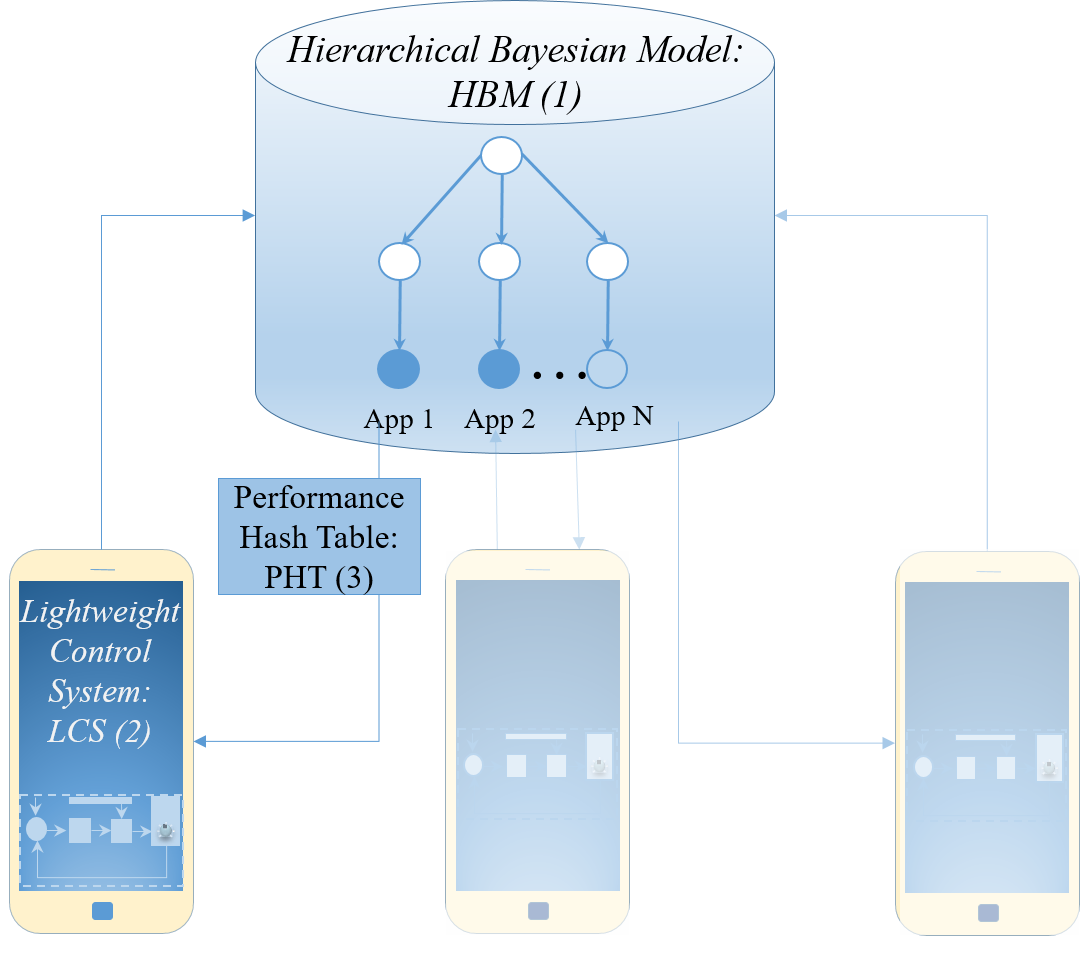
\includegraphics[width=\columnwidth]{figures/Mobile2.png}
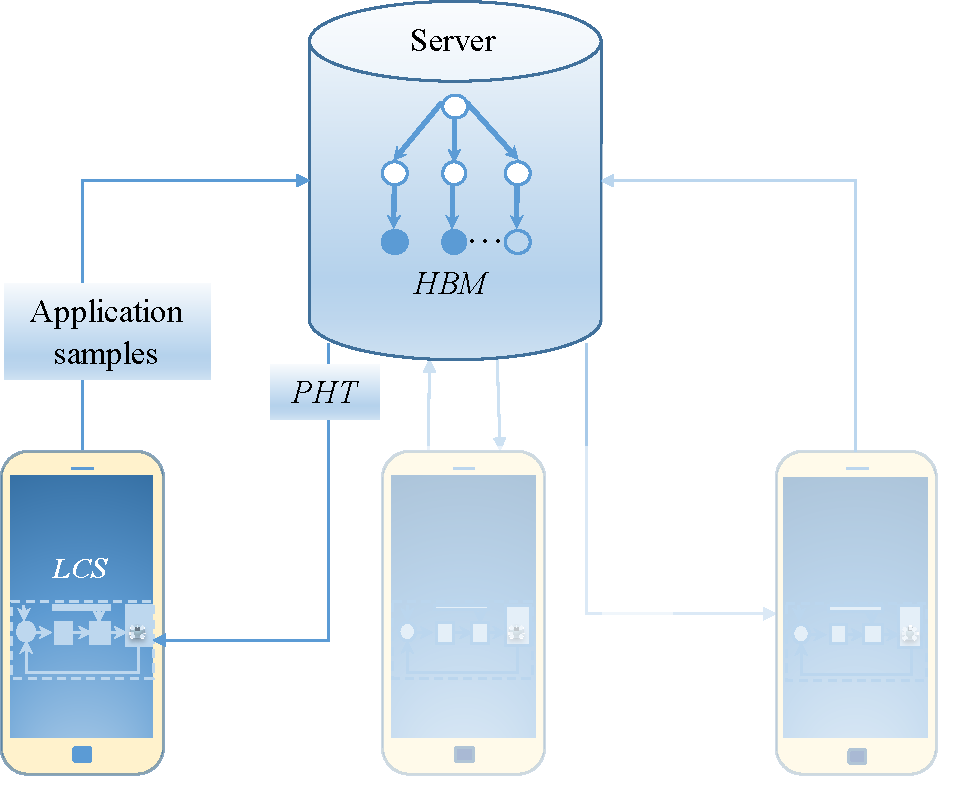
\includegraphics[width=\columnwidth]{figures/mobile-leo-poet2.pdf}
\caption{\SYSTEM{} overview: Mobile devices communicate with a server
  running a hierarchical Bayesian model (HBM) to learn
  performance/power tradeoffs.  The learned model is stored in a
  Performance Hash Table (PHT) and sent to a lightweight control
  system (LCS), which tunes the device's resource usage to meet
  performance goals with minimal energy. }
  \label{fig:overview}
\end{figure}
We therefore propose \SYSTEM{}\footnote{\textbf{C}ontrol \textbf{A}nd
  \textbf{L}earning for \textbf{O}ptimal \textbf{R}esource
  \textbf{E}nergy \textbf{E}fficiency}, a combination of learning and
control consisting of the three components shown in
\figref{fig:overview}: (1) a hierarchical Bayesian model (HBM) that
learns application-specific relationships between performance/power
and resource usage, (2) a lightweight control system (LCS) that
dynamically tunes resource usage to meet performance requirements with
minimal energy, and (3) a performance hash table (PHT), which is the
interface between learning and control.

\PUNT{
\SYSTEM{}'s design has two unique features:
\begin{itemize}
\item \textit{Remote Learning:} Sophisticated learning techniques
  produce accurate models of complicated systems but they are
  computationally expensive.  \SYSTEM{} mitigates this expense by
  running the learner on a remote server. This approach not only
  addresses overhead, it allows the learner to aggregate data from
  multiple devices, improving learning accuracy.
\item \textit{Fast Control:} The controller must not significantly
  impact performance or energy on the mobile device.  Yet, the
  controller must solve a constrained optimization problem to meet the
  performance goal with minimal energy.  To overcome this difficulty,
  \SYSTEM{}'s remote learner constructs a PHT for each application.
  While building the PHT is expensive, it allows the LCS to solve the
  constrained optimization problem in constant ($O(1)$) time.
\end{itemize}
}

\SYSTEM{}'s design has two unique features: \textit{Remote Learning}
and \textit{Fast Control}. First, sophisticated learning techniques
produce accurate models of complicated systems but they are
computationally expensive.  \SYSTEM{} mitigates this expense by
running the learner on a remote server. This approach not only
addresses overhead, it allows the learner to aggregate data from
multiple devices, improving learning accuracy. Second, the controller
must not significantly impact performance or energy on the mobile
device.  Yet, the controller must solve a constrained optimization
problem to meet the performance goal with minimal energy.  To overcome
this difficulty, \SYSTEM{}'s remote learner constructs a PHT for each
application.  While building the PHT is expensive, it allows the LCS
to solve the constrained optimization problem in constant ($O(1)$)
time.

\PUNT{ \SYSTEM{} overcomes three difficulties of combining learning
  and control:
\begin{itemize}
\item \textit{Model differences:} The learner produces non-linear
  models of discrete resources, while the control system is based on
  continuous, linear models.  \SYSTEM{} addresses this challenges by
  scheduling resources in time to map a continuous control into
  discrete resource configurations.
\item \textit{Learning overhead:} Sophisticated learning techniques
  produce accurate models of complicated systems but they are
  computationally expensive.  \SYSTEM{} overcomes this difficulty by
  running the learner on a remote server. This approach not only
  addresses overhead, it allows the learner to aggregate data from
  multiple devices, improving learning accuracy.
\item \textit{Control overhead:} The controller must not significantly
  impact performance or energy on the local device.  Therefore,
  \SYSTEM{} stores the learned models in the PHT, which allows it to
  schedule resources in constant ($O(1)$) time.  
\end{itemize}
The PHT is \SYSTEM{}'s key enabler.  It serves as the interface
between the HBM and LCS, allows the learner to be executed remotely,
and enables fast scheduling on the local device.  } \PUNT{ The main
challenge in combining a learning system with a control system is that
the learner produces non-linear models of resources (\eg cores and
clockspeeds) which are discrete, while the control system is based on
continuous linear models.  \SYSTEM{} bridges this gap by scheduling
resources in time to meet a performance requirement with minimal
energy.

The second challenge is that our learner (HBM) produces accurate
models of power and performance, but like many sophisticated machine
learning based models it is computationally expensive, so in \SYSTEM{}
the HBM runs on a remote server.  Moreover, as it is remote, it is
also capable of aggregating data from multiple devices, which makes
learner more powerful. The controller (LCS) runs on individual mobile
devices and receives models from the HBM.

Thirdly, for great user satisfaction, we would like this system to be fast. Hence, we propose that  these models are stored in the PHT, a data structure that allows the LCS to determine energy minimal resource schedules in constant time. The PHT is \SYSTEM{}'s key enabler.  While learning and control
systems exist, their combination requires an appropriate interface.
 %The PHT stores the learned models in such a way that this optimization problem can be solved in constant time, making it appropriate for use on a mobile device.   
While only tested with \SYSTEM{} we believe the PHT is general enough
to be used by different learning and control systems, or even to solve
different optimization problems.  }


% While control and learning frameworks exist, the key to combining
% them is creating an interface between the learning and control
% systems.  Specifically, learning frameworks for resource management
% map configurations (\eg{} resource allocations) into estimated
% performance and power.  These mappings are discrete and non-linear,
% capturing the behavior of the underlying system.  Controllers, in
% contrast, work with continuous linear models.  Therefore, our
% proposed combination of learning and control requires an interface
% to convert the discrete non-linear learned models into continuous
% linear models.  We address this challenge by forming the lower
% convex hull of points on the learned power/performance tradeoff
% space.  Interpolating between these points gives us a piecewise
% linear function that is appropriate for control models, yet still
% captures the significant behavior of the underlying system.  This
% interface allows us to combine the approaches studied in this paper,
% and we believe it is sufficiently general to apply to other
% combinations of learning and control as well.
\PUNT{ We test \SYSTEM{} on ARM big.LITTLE platforms with 20 different
  benchmarks to evaluate the HBM's ability to learn application
  specific models and the LCS's ability to deliver performance
  efficiently.  We compare to published learning and control methods
  in a variety of settings.  While many applications have inherent
  dynamics (\ie{}{} different processing phases), we explicitly test
  the ability to adapt to the unknown by running each application with
  other, random applications.}



We run HBM on an x86 server and the LCS on ARM big.LITTLE devices and
evaluate across 20 parallel benchmarks that exhibit a variety of power
nd performance trade-off behaviors.  We find that \SYSTEM{} delivers:
\begin{itemize}
\item \textbf{Reliable Performance: } \SYSTEM{} achieves an average
  error of 2\%, compared to 4.5-5.4\% for existing learning methods
  and 4.7\% for existing control approaches.
\item \textbf{Lower Average Energy:} \SYSTEM{} achieves an average
  energy consumption of only 7\% over optimal, compared to 25-52\% for
  existing learning methods and 26\% for existing control approaches.
\item \textbf{Better Worst Case Behavior:} \SYSTEM{}'s worst observed
  error across all applications and targets is 9\%, compared to
  19-73\% for prior learning methods and 25\% for existing control
  methods.  The worst observed energy for \SYSTEM{} is 1.82$\times$
  greater than optimal, while it is 4-12$\times$ greater for learning
  and 2.9 $\times$ greater for control.
\item \textbf{Adaptability to Dynamics:} We test \SYSTEM{}'s ability
  to deal with changing environments by introducing resource
  contention with other processes.  In a dynamically fluctuating
  environment, \SYSTEM{}'s worst performance error is 30\%, as
  compared to 71-84\% for prior learning approaches and 35\% for prior
  control approaches.
\end{itemize}

In summary, this paper makes the following contributions:
\begin{itemize}
\item Proposes \SYSTEM{}, a combination of a hierarchical Bayesian
  model with a lightweight control system, which addresses the twin
  challenges of \emph{complexity} and \emph{dynamics} to meet
  application performance goals with minimal energy on heterogeneous
  mobile systems.
\item An interface for combining learned models of discrete resource
  usage with continuous control models of resource dynamics that
  allows the lightweight controller to run in constant time.
\item Demonstrates that \SYSTEM{} achieves both smaller error and
  higher energy savings compared to independent learning and control
  techniques.
\end{itemize}
}